%!TEX root = ../mfilters.tex


\newcommand{\df}{\Delta f_{\text{дев}}}
\subsection{Зависимость отношения сигнал/шум на выходе согласованного
фильтра от параметров входного сигнала}

\subsection*{Рекомендации по анализу результатов эксперимента}
%\begin{itemize}
    %\item[$\times$] Сравнить времена корреляции шума на выходе фильтра и на входе.
%Для оценки времени корреляции шума на выходе использовать
%полученные графики 4.3 и 4.4 (это которые?). Сравнить время корреляции
%выходного шума с длительностью выходного сигнала, оценив эту
%длительность по графику 4.2. Пояснить утверждение о том, что
%шум на выходе является сигналоподобным.
    %\item[\checked]Почему отношение сигнал/шум не зависит от девиации и прямо
    %пропорционально длительности входного импульса?

    %\item[$\times$] Качественно нарисовать график зависимости отношения
    %сигнал/шум от длительности входного сигнала для прямоугольного
    %видеоимпульса. Как изменится зависимость по сравнению с
    %аналогичной, построенной для ЛЧМ сигнала? Сравнить поведение
    %усредненных кривых и случайный разброс экспериментальных
    %точек относительно усредненной кривой.

%\end{itemize}

\subsubsection{Изменяющаяся длительность ЛЧМ сигнала}%


\label{ssub:izmeniaiushchaiasia_dlitel_nost_signala_tau_}

\begin{figure}[h!]
    \centering
    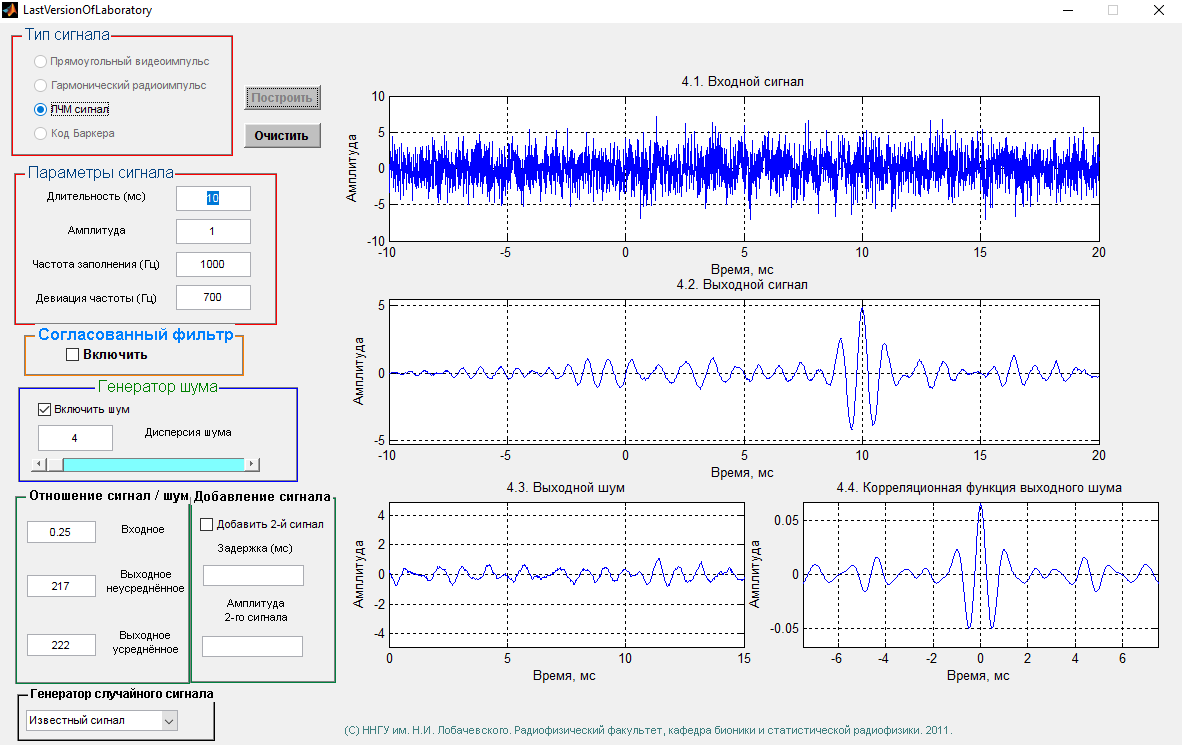
\includegraphics[width=\linewidth]{python/task4/t4s4_10_0}
    \caption{Панель виртуального прибора для задания 4.}
    \label{fig:4.1}
\end{figure}

Установили девиацию частоты $\Delta f_{\text{дев}}= 700$ Гц и изменяли
длительность в пределах 10 мс -- 100 мс. 


Был проведен эксперимент, в котором для нескольких реализаций виртуальным
прибором\footnote{Виртуальному прибору -- виртуальный студент}
вычислялось усредненное и неусредненное отношение сигнал/шум. Получившееся
облако точек представлено на рис.\ref{fig:4.1}.



\begin{figure}[h!]
    \centering
    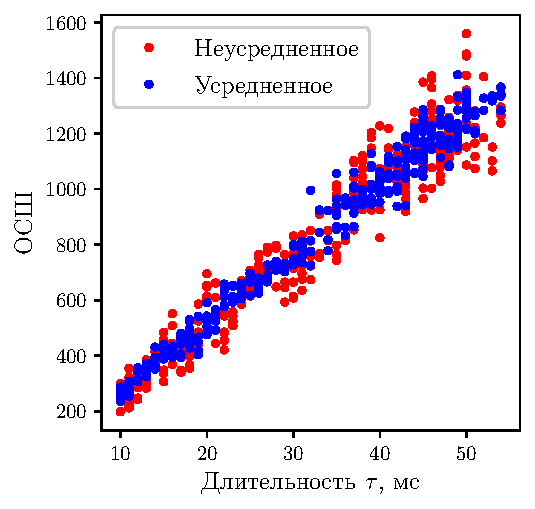
\includegraphics[width=0.6\linewidth]{imgs/task4/t4f1} 
    \caption{Облако значений зависимости ОСШ от длительности $\tau$ ЛЧМ
    сигнала. Красными точками на графике отмечено ОСШ посчитанное по одной
    реализации, синими точками -- ОСШ усредненное за 10 реализаций }
    \label{fig:4.1}
\end{figure}


\newcommand{\mSNR}{\overline{\text{ОСШ}}}
Между реализациями, полученными при одинаковом значении длительности $\tau$
усреднялись, вычислялось среднее значение и формировалась усредненная функция
$\mSNR$. Зависимость усредненного 
$\mSNR(\tau)$ от длительности сигнала представлена на рис. \ref{fig:4.2}.




\begin{figure}[h!]
    \centering
    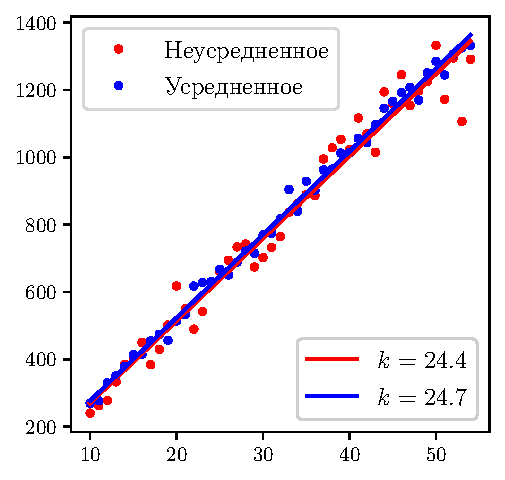
\includegraphics[width=0.6\linewidth]{imgs/task4/t4f2}
    \caption{Усредненная зависимость $\mSNR$ от длительности $\tau$ ЛЧМ
        сигнала. Усреднение производилось по 100 реализациям для каждого
        значения длительности сигнала.  Сплошной линией показана линейная
        аппроксимация получившейся зависимости. Коэффициент $k$ обозначает
        коэффициент наклона прямой}
    \label{fig:4.2}
\end{figure}

\subsubsection{Изменяющаяся девиация частоты ЛЧМ сигнала}%
\label{ssub:izmeniaiushchaiasia_deviatsiia_chastoty_signala}
Установили длительность сигнала $\tau=50$ мс и изменяли девиацию в пределах
400 Гц - 1000 Гц.

Для одной реализации сигнала виртуальным прибором
вычислялось отношение сигнал/шум. Получившаяся зависимость приведена на рис.
\ref{fig:4.3}.

\begin{figure}[h!]
    \centering
    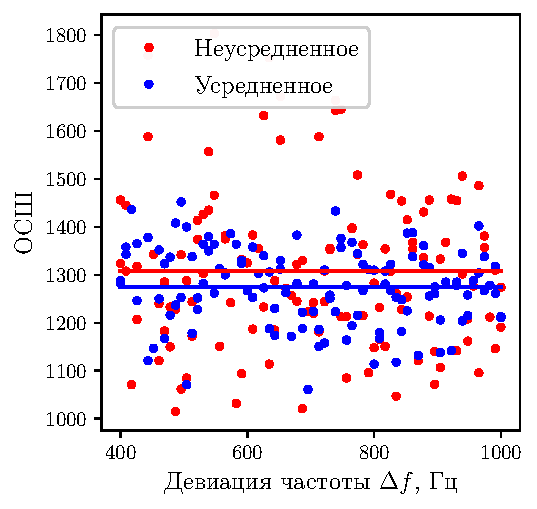
\includegraphics[width=0.6\linewidth]{imgs/task4/t4ff1}
    \caption{Облако значений ОСШ от девиации частоты $\Delta f$ ЛЧМ
        сигнала. Усреднение производилось по 10 реализациям для каждого
        значения ОСШ}
    \label{fig:4.3}
\end{figure}

\subsubsection{Анализ экспериментальных данных}%
\label{sub:analiz_eksperimenta}

Стоит обратить внимание на то, что шум из дельта-коррелированного превратился в
сигнало-подобный. Это связано со способом фильтрации: оптимальный фильтр
пропускает гармоники, соответствующие спектру сигнала. 

В \cite{doc} показано, что мощность СПМ шума на выходе коррелятора будет равна
\begin{equation}
    S_\eta(\omega) = \abs{K(j\omega)}^2 S_\xi (\omega), \text{ где}
\end{equation}
$S_\xi(\omega)$ -- спектральная плотность мощности шума на входе в систему
$\abs{K(j \omega)}$ -- коэффициент передачи согласованного фильтра.

%Сравним времена корреляции выходного шума с длительностью входного сигнала.


Как известно максимальное ОСШ на выходе линейной системы можно представить в
виде
\begin{equation}
    \label{eq:maxsnr}
    \rho_{\text{вых}} \leq \frac{1}{2\pi} \int\limits_{-\infty}^{\infty}
    \frac{\abs{C_m (j \omega)}^2}{S_\xi(\omega)} \dd \omega, \text{ где}
\end{equation}
$C_m(j \omega)$ -- амплитудный спектр сигнала, . Поскольку в данной работе модель шума выбрана белой, то
$S_\xi(\omega) = \mean{\xi}$, где  $\mean{\xi}$ -- дисперсия белого шума.

Из теории также известно, что амплитудный спектр ЛЧМ-импульса с большой базой
$B= \frac{\tau \abs{\Delta f_{\text{дев}}}}{2 \pi}\gg 1$ можно
считать прямоугольным и равным 
\begin{equation}
    \abs{C_m(j \omega)}^2 = \frac{\epsilon_m}{2 \Delta f_{\text{дев}}} = \frac{\tau}{4
    \df}, \text{ при } \omega_0 - \frac{\df}{2} \leq \omega \leq \omega_0 +
    \frac{\df}{2}
\end{equation}

Интегрируя выражения \eqref{eq:maxsnr} получаем
\begin{equation}
    \label{eq:maxsnr_simplified}
    \rho_{\text{вых}} \leq \frac{1}{2\pi} \cdot \frac{\tau}{4}
\end{equation}

Из \eqref{eq:maxsnr_simplified} следует, что ОСШ линейно зависит только от
длительности импульса на выходе системы. Это и подтверждают экспериментальные
графики рис. \ref{fig:4.2} и рис. \ref{fig:4.3}







